\section{Overview}\label{sec:overview}
In this section, we give an overview of our approach with the aid of a motivating example.

\subsection{Smart Contract Vulnerabilities}\label{sec:overview-vul}

A security analyst, Alice, can specify various types of vulnerabilities that may appear
in a smart contract. 
% For instance, a \emph{Reentrancy vulnerability}~\cite{attack1} 
% occurs when an attacker's previous invocation is allowed to make new calls to the 
% victim contract before the previous execution is complete. This means that if the 
% call involves money transactions, the attacker can repeatedly 
% trigger many transactions until the current procedure runs out of gas. 
% A \emph{Timestamp dependence vulnerability}~\cite{attack-time}, on the other hand, 
% happens when a transaction relies on a certain timestamp, which allows malicious miners to gain advantage by choosing a suitable timestamp. 
For instance, Figure~\ref{fig:motivate} shows a simplified example of a
\reentrancy attack. The \texttt{withdraw} function does two
steps: \circled{1} send a given amount of Ether to the caller, and \circled{2}
update the storage state to reflect the new balance. At any point, the total
amount of balances of the victim and attacker should remain the same (i.e.,
$B_v+B_a=C$). However, since \circled{1} happens before updating the state in
\circled{2}, an attacker can re-enter the \texttt{withdraw} function again
through the anonymous callback function triggered by \circled{1}. As a result,
the execution of the attack program can lead to an inconsistent state (i.e.,
$B_v' + B_a' > C$), which enables the attacker to extract a large amount of
Ether from the victim.\footnote{Ethereum's gas mechanism ensures that this
callback loop terminates.}\looseness=-1 

To automatically generate exploits for the \reentrancy vulnerability, Alice
first specifies a \emph{query} that \emph{characterizes} the semantics of
\reentrancy. As shown in the lower part of Figure~\ref{fig:motivate}, the attack
can be summarized using a sequence of key statements between the victim and the
attacker, i.e., two or more \texttt{call} instructions followed by a
\texttt{store} operation, which can be expressed using the first-order
formula in Figure~\ref{fig:motivate}.

% This section uses the most recent \batchoverflow 
% vulnerability (CVE-2018–10299)~\cite{attack-int} as a motivating example.
% Exploits due to this vulnerability have resulted in the creation of 
% trillions of \emph{invalid} Ethereum Tokens in 2018~\cite{batch-news}, causing major exchanges to temporary halt until all tokens could be reassessed.
% As shown in Figure~\ref{fig:batchcode}, the \texttt{batchTransfer} function 
% performs a multiplication that can overflow 256 bits, 
% which results in a small value that passes the check at line 12 and 
% further transfers a large amount of tokens to the attacker (line 20).\looseness=-1

% \begin{lstlisting}[xleftmargin=.2\textwidth]      
% $\exists\ arg_0, arg_1, r_1, r_2, r_3, call$ 
% (&& (= $r_3$ ($\otimes$ $r_1$ $r_2$)) 
%     (> $\geval{r_2}$ $\geval{r_3}$)
%     (interfere? $r_2$ call.value) 
%     (interfere? $arg_0$ call.addr) 
%     (interfere? $arg_1$ call.value)) 
% where $\otimes \in${+,$\times$}
% \end{lstlisting}


% \begin{figure}
%     \begin{lstlisting}[xleftmargin=0em,linewidth=6cm]  
% $\exists\ arg_0, arg_1, r_1, r_2, r_3, call$ 
% (&& (= $r_3$ ($\otimes$ $r_1$ $r_2$)) 
%     (> $\geval{r_2}$ $\geval{r_3}$)
%     (interfere? $r_2$ call.value) 
%     (interfere? $arg_0$ call.addr) 
%     (interfere? $arg_1$ call.value)) 
% where $\otimes \in${+,$\times$}
%       \end{lstlisting}
%   \caption{Query for the BatchOverFlow}
%     \label{fig:sum-gen}
%   \end{figure} 
%   \begin{figure}
%     \begin{lstlisting}[xleftmargin=1em,linewidth=5.5cm]     
% batchTransfer($arg_0$, $arg_1$) {
%   ... 
%   $r_3$ = $r_1$ $\otimes$ $r_2$;
%   ... 
%   call(gas, addr, value, ...);
%   ...
% }
%       \end{lstlisting}
%     \caption{The key pattern of the BatchOverflow Vulnerability}
%     \label{fig:batchcode}
% \end{figure}
\begin{figure}[!t]
  \centering
  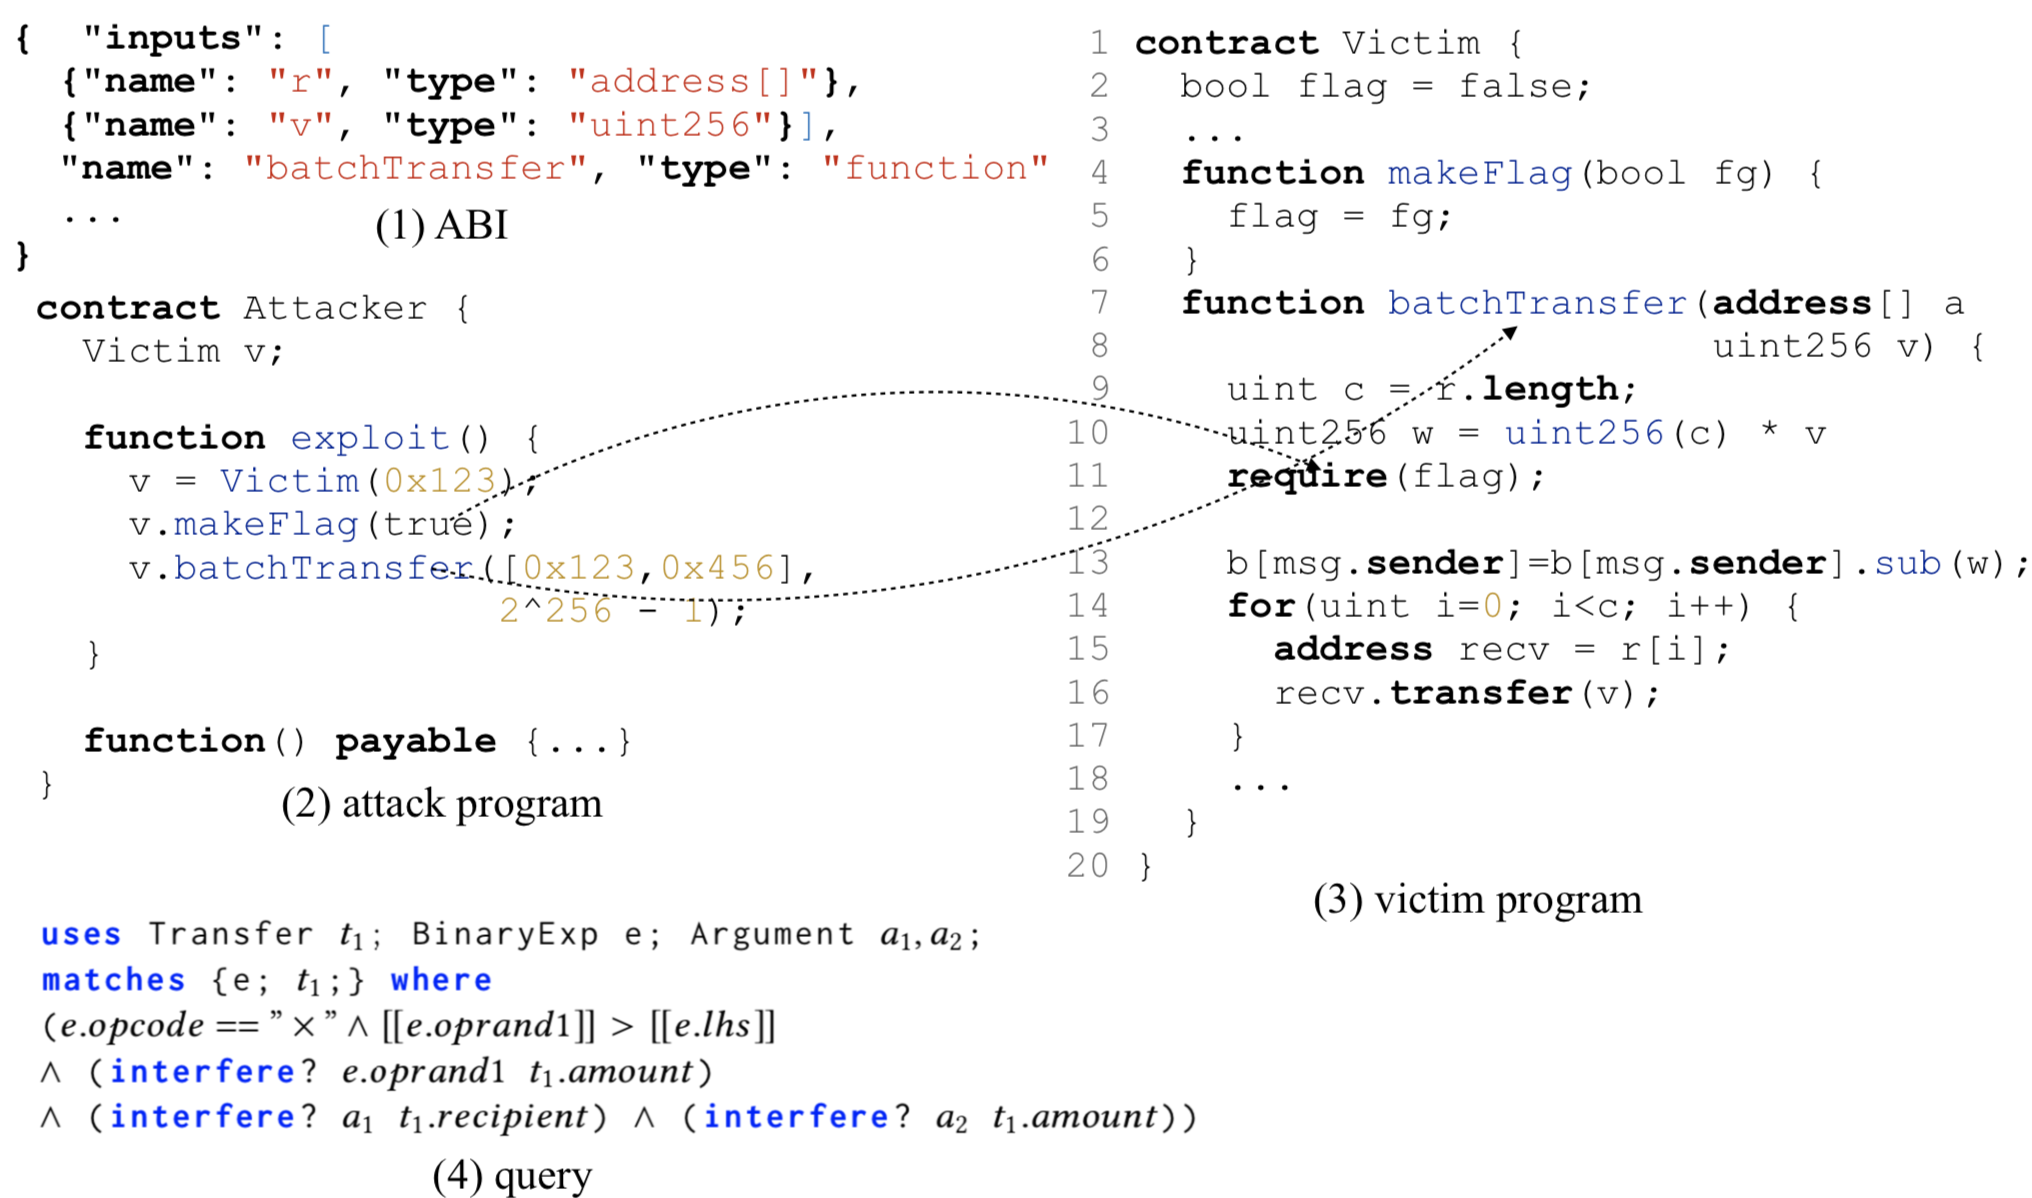
\includegraphics[scale=0.23]{batchoverflow.png}
\caption{An example to show the \batchoverflow attack.}
\label{fig:batchcode}
% \vspace{-0.2in}
\end{figure}
% \toolname's specifications are assertions expressed in the Racket 
% language~\cite{racket}. In particular, the \batchoverflow vulnerability
% can be expressed as the query in Figure~\ref{fig:batchcode}. To highlight 
% the key concepts in our query language,
% we also visualize this vulnerability pattern in Figure~\ref{fig:batchcode}. 
% Here, $arg_i$, $r_j$, and \texttt{call} represent function arguments, 
% registers, and the \texttt{CALL} instruction (to perform a transaction in Solidity), respectively. 
% We use $\geval{r_i}$ to denote the value 
% (either concrete or symbolic) in the register $r_i$.
% The \texttt{interfere?} function, which is defined
% in section~\ref{sec:problem}, checks the interference between two 
% expressions. The interference~\cite{non-interfere} 
% (denoted by an arrow in Figure~\ref{fig:batchcode}) in our system precisely
% captures the data- and control-dependency. For instance,   
% the vulnerability states that, there exists a \texttt{CALL} instruction
% for which the beneficiary (i.e., recipient's address) and value are controlled by the attacker (line 5, 6).
% Furthermore, the transaction's value is influenced by a register (line 4) used in an arithmetic operation that overflows (line 2,3).

% We leverage the constraint solver Z3. Yet we cannot
% simply pass our set of collected constraints as is, as the
% constraint solver is unaware of the special semantics of
% Keccak-256 results and symbolic-read objects.
Once Alice expresses the \reentrancy vulnerability, the next step is to
construct an attack to confirm that the vulnerability indeed exists in the
victim contract. Alice can leverage existing symbolic execution
tools~\cite{mythril,oyente,teether} to generate exploits for simple properties such as 
attack-control~\cite{teether}) in a \emph{single contract}. But for
complex vulnerabilities that require reasoning about interactions among multiple
contracts (e.g., attacker versus victim in \reentrancy or caller versus callee in
Parity Multisig~\cite{multisig}), existing tools provide either no 
support~\cite{teether} or very limited support that 
leads to high rates~\cite{oyente} of false positives and negatives (as shown in
Section~\ref{sec:oyente}). % due to the increasing search space imposed by multiple contracts. 
Yet Alice can easily initialize the boilerplate code
for basic interactions, like the ``attack template" on the left hand side of
Figure~\ref{fig:motivate}. What she needs is an efficient way to  
fill in the details of the attack program, which involves exploring the space 
of all programs that can be obtained by completing the template with the methods 
from the victim's interface.
% Doing so manually is challenging, however, because the analyst has to understand the semantics of the smart contract and simulate all possible interactions that an attacker may perform.  As a result, the analysis process is both tedious and error-pone.
% has to figure out the following details:
% \begin{itemize}
% \item Figure out a list of public methods from the Application Binary Interface (ABI)
% of the victim contract~\ref{fig:attack-abi}. 
% \item Construct attack candidates by trying all possible combinations of function
% calls up to size $K$. Note that even for this simple benchmark with only 16 public
% methods, there are already 65536 candidates of size 4!
% \item For each candidate from the previous step, she has to execute it and manually
% check if there is any trace satisfying the constraint of the vulnerability. Note that
% the number of traces will be exponential to the number of branches of each candidate.
% \end{itemize}
% Since the entire process is tedious and error-pone, as the vulnerabilities get more 
% complex and the size of the benchmarks become larger,
% it becomes more difficult to construct the attack programs manually.
% \begin{figure}
%     % \centering
%     \begin{subfigure}[b]{0.4\textwidth}
%     \begin{lstlisting}[escapechar=@]  
% contract PausableToken {
% bool flag = false; 

% function makeFlag(bool fg) { 
%  flag = fg; 
% } 

% function batchTransfer(address[] _receivers, uint256 _value) {
%     uint cnt = _receivers.length;
%     uint256 amount = @\textbf{uint256(cnt) * _value}@;
%     require(@\textbf{flag}@);
%     require(balances[msg.sender] @\textbf{>= amount)}@;

%     balances[msg.sender] = 
%       balances[msg.sender].sub(amount);
%     for (uint i = 0; i < cnt; i++) {
%       address recv = _receivers[i];
%       balances[recv] = 
%         balances[recv].add(_value);
%       @\textbf{Transfer(msg.sender, recv, _value)}@;
%     }
%     return true;
%   }
% }
% \end{lstlisting}
%     \caption{The Vulnerable Program}
%       \label{fig:attack-vic}
%     \end{subfigure} \\
%     \begin{subfigure}[b]{0.4\textwidth}
%     \begin{lstlisting}      
%   contract Attacker {
%     ...
%     function exploit() {
%       VulContract v;
%       v.makeFlag(true);
%       v.batchTransfer([0x123, 0x456], $2^{256} - 1$);
%     }
%   }
% \end{lstlisting}
%     \caption{An Attack Program}
%       \label{fig:attack-code}
%     \end{subfigure} \\
%     \begin{subfigure}[b]{0.4\textwidth}
%     \begin{lstlisting} 
%  {
%   "inputs": [
%   {"name": "_receivers", "type": "address[]"},
%   {"name": "_value", "type": "uint256"}
%   ],
%   "name": "batchTransfer", "type": "function"
%   ...
% },{ 
%  "inputs": [{"name": "fg", "type": "bool"}],
%  "name": "makeFlag", "type": "function"}
%   \end{lstlisting}
%       \caption{Contract Application Binary Interface (ABI) for the vulnerable contract in Fig~\ref{fig:attack-vic}}
%       \label{fig:attack-abi}
%     \end{subfigure}
% \caption{A running example to show the \batchoverflow Vulnerability\label{fig:overview-example}}
% \end{figure}

\subsection{\toolname}
\vspace{-0.04in}
\toolname helps automate this process by searching for attacks that exploit a
given vulnerability in a victim contract. The tool takes as input a potential
vulnerability $\vulnerability$ expressed as a declarative specification. If
$\vulnerability$ exists in the victim contract, \toolname\ automatically
synthesizes an \emph{attack program} that exploits $\vulnerability$. An attacker
interacts with a vulnerable contract through its public methods defined in the
ABI. Therefore, our goal is to construct an attack program that exploits the
victim's ABI and that contains at least one concrete trace where
$\vulnerability$ holds. 

To achieve this goal, \toolname  models 
the executions of a smart contract as \emph{state transitions} over registers, memory, and storage. 
The vulnerability $\vulnerability$ 
is expressed in Racket~\cite{racket} as a boolean predicate over these state transitions. 
The technical challenge addressed by \toolname is to efficiently search for an attack program where $\vulnerability$ 
holds. 

To illustrate the difficulty of this task, consider the problem of synthesizing an attack 
program that exploits 
the \batchoverflow vulnerability (CVE-2018–10299)~\cite{attack-int} in Figure~\ref{fig:batchcode}. 
The attack program performs a complex three-step 
interaction with the victim contract.  First, the attacker must set the storage variable 
\texttt{flag} to \texttt{true} to pass the check at line 12. Next, it needs to 
assign a large number to \texttt{v} that leads to an overflow at line 11. 
Finally, it specifies the attacker's address as the beneficiary of the transaction (line 17). 
Synthesizing this attack program involves discovering which methods to call, in what order, and with what arguments. 

%Given those requirements,
%one straightforward way is to use an off-the-shelf constraint solver to 
%generate a counter-example as the attack~\cite{oyente}. 
%However, since a constraint solver does not understand the special semantics 
%in smart contracts, such as the
%Keccak-256 hash functions and symbolic-read over storage, the naive approach will lead to poor coverage and fail to find
%the desired attack. To bypass this limitation, one way is to simulate an real attacker's behavior which constructs the 
%attack program through a sequence of calls to the public methods.

The naive approach to solving this problem is to generate 
all possible \emph{concrete programs} and explore the space of 
their \emph{concrete traces}. This approach suffers from two sources of exponential explosion. 
First, there are $O(n^k)$ concrete programs of length $k$ for a victim contract with $n$ public methods.  
Second, the number of concrete traces in each of these programs is exponential in the size of the 
program's global control-flow graph obtained by inlining all method calls. 

To address the trace explosion challenge, \toolname\ employs a novel summary-based 
symbolic evaluation technique presented in Section~\ref{sec:sum}. Intuitively,
this technique enables \toolname to preserve only those state transitions that 
are persistent across different transactions and are \emph{sufficient} to answer
the vulnerability query.\looseness=-1

To address the program explosion challenge, Section~\ref{sec:impl} introduces three additional 
optimizations. First, instead of exploring the space of concrete programs, we
leverage \rosette~\cite{rosette} to partition this space into a small set of 
\emph{symbolic programs} 
(Section~\ref{sec:rosette}). 
% Second, instead of eagerly exploring the space of
% symbolic programs,  we design a simple but effective \emph{early pruning}
% strategy that allows \toolname to prune \emph{infeasible} symbolic candidates
% before executing them (Section~\ref{sec:prune}). 
Second, instead of executing
each symbolic program \emph{sequentially}, we partition the search space by case
splitting on the range of symbolic variables, which enables \toolname to
simultaneously explore multiple symbolic candidates
(Section~\ref{sec:parallel}).
